\documentclass{beamer}
\usetheme{Warsaw}

\usepackage[utf8]{inputenc}
\usepackage{fancybox}
\usepackage{multimedia} 
\usepackage{subfig}
\usepackage{amsmath}
\usepackage{hyperref}
\usepackage[all]{xy}
\begin{document}


\title[Angewandte Mathematik] % (optional, only for long titles)
{Angewandte Mathematik
\\
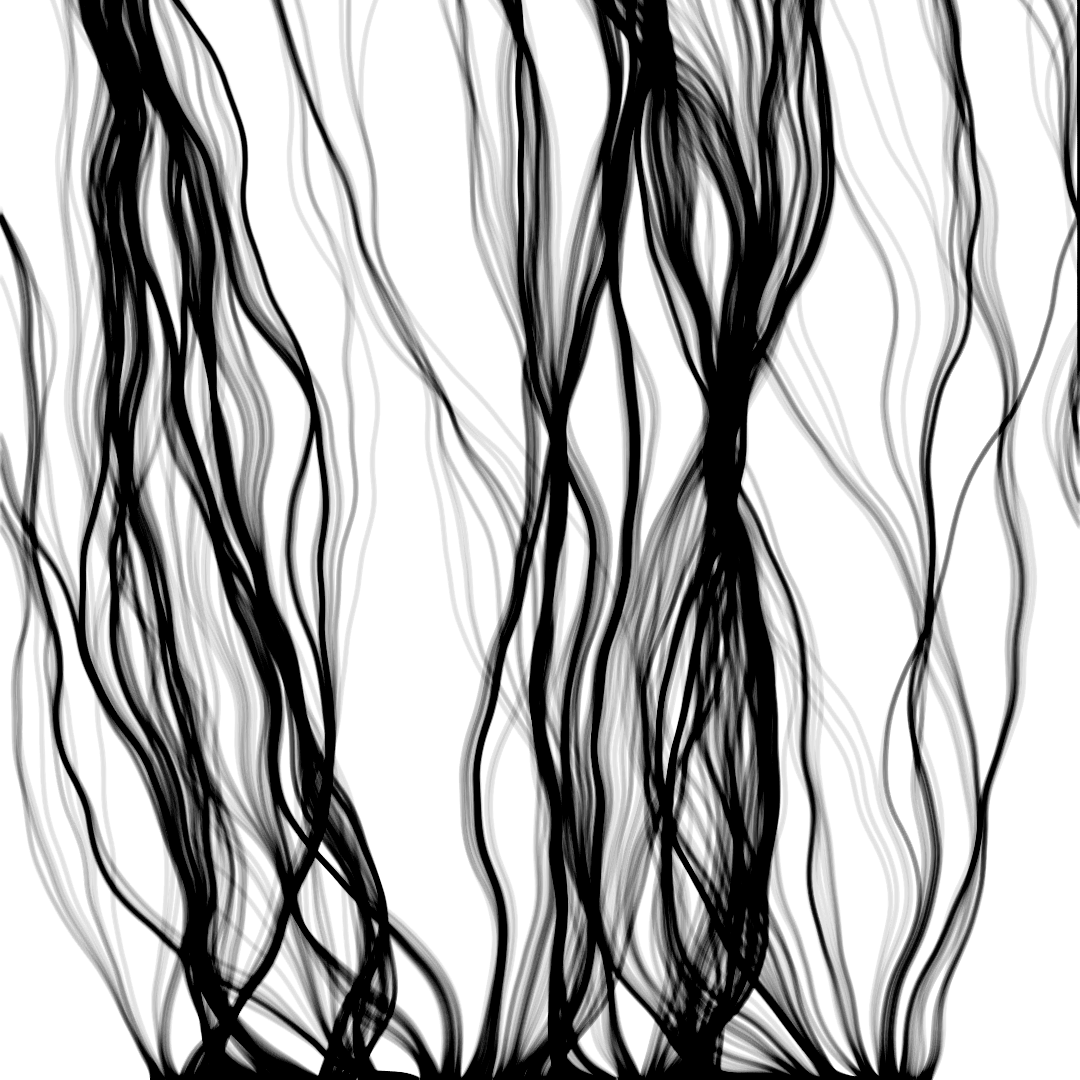
\includegraphics[scale=0.15]{images/cover}
}
\subtitle{}
\author[Dr. Johannes Riesterer] % (optional, for multiple authors)
{Dr.  rer. nat. Johannes Riesterer}

\date[KPT 2004] % (optional)
{}

\subject{Angewandte Mathematik}

\frame{\titlepage}

\begin{frame}
    \frametitle{Angewandte Mathematik}
\framesubtitle{}
    \begin{block}{Symmetrische Matrix}
Eine Matrix $A$ heißt symmetrisch, falls $A^t = A$ gilt.
\end{block}

\begin{block}{Spektralsatz}
Eine symmetrische Matrix $A$ ist diagonalisierbar, d.h es gibt eine invertiertere Matrix $B$ mit 
\begin{align*}
B^{-1}A B = \begin{pmatrix}    \lambda_{1} & & \\
    & \ddots & \\
    & & \lambda_{n}\end{pmatrix}
\end{align*}
wobei $\lambda_1, \cdots \lambda_n$ die Eigenwerte der Matrix $A$ sind. 
\end{block}

 \end{frame}

\begin{frame}
    \frametitle{Angewandte Mathematik}
\framesubtitle{}


    \begin{block}{Haupminoren}
Für $A = (a)_{i \leq n,j \leq n}$ ist der $k$-te Hauptminor $M_k(A)$ definiert durch 
\begin{align*}
M_k(A) := \det(a)_{i \leq k, j \leq k}
\end{align*}

\end{block}

 \end{frame}



\begin{frame}
    \frametitle{Angewandte Mathematik}
\framesubtitle{}
    \begin{block}{Positiv definite  Matrix}
Eine Matrix $A$ heißt positiv definit, falls $x^t Ax > 0$ und negativ definit, falls  $x^t Ax < 0$ für alle $x \neq 0$ gilt.
\end{block}

    \begin{block}{Positiv definite und symmetrische  Matrix}
Für eine symmetrische Matrix $A$ sind die folgenden Aussagen Äquivalent:
\begin{itemize}
\item $A$ ist positiv  (negativ) definit.
\item Die Eigenwerte $\lambda_1, \cdots \lambda_n$ von $A$ sind positiv (negativ).
\item Die Hauptminoren $M_k(A) > 0$ für alle $1 \leq k \leq n$ von $A$ sind positiv, bzw  alternierend, also $(-1)^k M_k(A) > 0$ für alle $1 \leq k \leq n$ 
\end{itemize}

\end{block}



 \end{frame}

\end{document}

